\documentclass[11pt,a4paper]{article}
\usepackage[margin=2.2cm]{geometry}
\usepackage{amsmath,amssymb}
\usepackage{graphicx}
\usepackage{booktabs}
\usepackage{array}
\usepackage[hidelinks]{hyperref}
\usepackage{caption}
\usepackage{enumitem}
\usepackage{microtype}
\graphicspath{{../figures/}}
\setlength{\parskip}{4pt}
\setlength{\parindent}{0pt}
\title{On-blade induced drag of curved lifting lines in the Vortex Step Method:\\
problem statement, literature, and a parameter-free regularisation}
\author{Working document, awegroup/Vortex-Step-Method, branch \texttt{feature/curved-bound-vortex-regularisation}}
\date{17 September 2026 (rebuilt 12 October 2026)}

\begin{document}
\maketitle

\begin{abstract}
The \texttt{develop} branch of the Python Vortex Step Method (VSM) was aligned with the coupling rules of Gaunaa, Li and Pirrung (TORQUE 2026): force magnitudes from the three-quarter-chord flow, force directions from the quarter-chord flow, and a Kutta--Joukowski force on the attached-trailed vortex legs. With these rules the on-blade induced drag equals the Trefftz-plane value exactly on straight wings, but on the TU~Delft V3 kite it is 7--15\,\% low and decreases without bound as the number of spanwise panels increases. This document states the problem, identifies its cause (the logarithmically singular self-induction of the curved bound vortex, evaluated on its own line to set the force direction, entering the drag through $\rho\Gamma\,u\sin\alpha$), reviews how the literature treats the singularity, tests the two published remedies inside the VSM framework, and describes the parameter-free regularisation now implemented: the quarter-chord velocity is built from the classical lifting-line downwash of the wing unrolled onto the local tangent line, plus the difference between the actual and the unrolled vortex systems with the bound vorticity and the leg starting points spread chordwise with the thin-airfoil distribution. The result is identically zero on straight wings, mesh-independent, and within 1\,\% of the Trefftz-plane induced drag on an arc wing, a swept wing, the swept--anhedral elliptic wing of Gaunaa et al., and the V3 kite. All tables are reproduced by \texttt{docs/validation/curved\_bound\_vortex\_validation.py}.
\end{abstract}

\section{Status of the implementation with respect to Li and Gaunaa}
\label{sec:status}

The \texttt{develop} branch (commits \texttt{233a238}\ldots\texttt{62c53af}) implements the following elements of Gaunaa, Li and Pirrung~\cite{gaunaa2026} and Li, Gaunaa, Pirrung and L{\o}nb{\ae}k~\cite{li2026}:
\begin{itemize}[nosep]
  \item CP1: the inner 2D velocity is the component perpendicular to the local quarter-chord line, and the chord is measured perpendicular to that line;
  \item TAT1: the section's own 2D bound-vortex induction is subtracted at the three-quarter-chord point (the VSM \texttt{subtract\_bound\_2D} term, which the code has had since its inception);
  \item TAT2: force magnitudes from the three-quarter-chord angle of attack, with $\Gamma_i = \tfrac12 |V_{\mathrm{inner},i}|\, c_i\, C_l(\alpha_{3/4,i})$ (eq.~4 of~\cite{gaunaa2026});
  \item TAT3: force directions from the undisturbed relative flow at the quarter chord (\texttt{is\_aoa\_corrected=True}, now the default);
  \item the attached-trailed (AT) vortex force $\rho\,\Delta\Gamma_j\, \mathbf V_{3D,\mathrm{rel},j}\times \mathbf l_{AT,j}$ evaluated at the three-quarter-chord point of the leg;
  \item the implicit artificial viscosity with the tip closures and the relaxation-factor bound of~\cite{li2026}, the latter halved for the VSM after measurement of the fixed-point Jacobian.
\end{itemize}

\textbf{Two elements do not follow the published prescription.}
\begin{enumerate}[nosep]
  \item \emph{The curved bound-vortex influence on the direction velocity.} Reference~\cite{gaunaa2026} states that LL-Gaunaa includes ``the influence of the curved bound vortex'' according to~\cite{li2020}. In~\cite{li2020} (Section~2.2) that influence is the induction of the 3D bound vortex minus that of an infinitely long 2D vortex of the section's own strength, evaluated at the \emph{three-quarter} chord, assumed constant along the chord, and added to the quarter-chord velocity. \texttt{develop} instead evaluated the other panels' bound segments \emph{on the quarter-chord line itself} (commit \texttt{9c43c1a}), which~\cite{li2020} calls LL-P\&S and shows to be log-singular and non-convergent. This is the cause of the problem treated here (Section~\ref{sec:problem}). A literal implementation of the~\cite{li2020} recipe in this code was also tested and fails on straight wings (Section~\ref{sec:lit}); the 2026 paper and its online appendix~\cite{appendix2026} do not specify the quarter-chord term further, so the form used in the authors' code needs clarification with them. The branch replaces the term by the regularisation of Section~\ref{sec:fix}.
  \item \emph{The direction of the attached-trailed legs.} Reference~\cite{gaunaa2026} aligns the bound part of the trailed vortex with the local chordwise direction, i.e.\ perpendicular to the quarter-chord line (CP1). The code keeps the legs along the section ribs; the panel frame, the chord and the three-quarter-chord control point do follow CP1. On the V3 the two directions differ by up to 0.77 in chord-to-span skew at the tips. Perpendicular legs were compared again with the regularisation of Section~\ref{sec:fix} in place (Section~\ref{sec:legs}): they cannot be built on a kinked planform (adjacent perpendiculars cross and the solve returns NaN), they lower the V3 lift by 6\,\% and worsen the comparison with RANS (mean $|\Delta C_L|$ 0.031 instead of 0.020), and with the attached-trailed force the on-blade induced drag sits 2.5--4\,\% above the Trefftz plane, whereas rib legs sit within 1.5\,\%. (The authors' own swept wings show a discrepancy of the same size but of the opposite sign: on-blade induced drag 1--5\,\% \emph{below} the Trefftz plane, Table~2 of~\cite{gaunaa2026} and the appendix~\cite{appendix2026}; their VLM reference is 3\,\% below as well.) The ribs are kept. This remains a documented deviation; the regularisation works with either leg direction.
\end{enumerate}

\section{Problem statement}
\label{sec:problem}

\subsection{Observation}
For steady, uniform inflow the induced drag can be computed in two ways from the same converged circulation $\Gamma(s)$: on the blade, by projecting the panel forces (lift tilted by the quarter-chord flow angle, plus the AT force) onto the freestream, or in the Trefftz plane from the momentum in the far wake. The Trefftz value depends only on $\Gamma(s)$ and the wake geometry; for a consistent force evaluation the two must agree. Table~\ref{tab:conv} shows the ratio for inviscid polars ($C_l = 2\pi\alpha$) with the bound segments evaluated on the line.

\begin{table}[h]\centering\small
\caption{On-blade over Trefftz-plane induced drag, bound segments on the quarter-chord line (\texttt{develop} as of \texttt{62c53af}), inviscid polars.}
\label{tab:conv}
\begin{tabular}{lcccccc}
\toprule
case & $N=10$ & 20 & 40 & 80 & 160 & trend\\
\midrule
straight rectangular, AR 8 & -- & 1.000 & 1.000 & 1.000 & -- & exact\\
swept $30^\circ$, AR 8, streamwise ribs & 0.933 & 0.937 & 0.939 & 0.940 & 0.936 & converged, 6\,\% low\\
circular arc, $110^\circ$, $R=4c$ & 0.998 & 0.977 & 0.957 & 0.937 & 0.917 & $-0.02$ per doubling\\
elliptic, 10\,\% sweep, 25\,\% anhedral (\cite{gaunaa2026}) & -- & -- & 0.980 & 0.967 & 0.954 & $-0.013$ per doubling\\
V3 kite, CAD geometry & -- & 0.933 & 0.907 & 0.881 & 0.854 & $-0.026$ per doubling\\
\bottomrule
\end{tabular}
\end{table}

Lift is converged to four digits in all cases; only the drag drifts. The drift is a clean logarithm in $N$ on every wing with out-of-plane curvature.

\subsection{Cause}
The quarter-chord direction velocity of panel $i$ was assembled as
\begin{equation}
\mathbf V_{1/4,i} = \mathbf V_\infty + \sum_j \Gamma_j\,\mathbf K^{\mathrm{trailed}}_j(\mathbf P_i) + \sum_{j\neq i} \Gamma_j\, \mathbf K^{\mathrm{bound}}_j(\mathbf P_i),
\label{eq:current}
\end{equation}
with $\mathbf P_i$ on the bound line. The last sum is needed: without it a swept wing with streamwise legs diverges (ratio 0.43 at $N=40$, 0.25 at $N=160$), because the legs carry a logarithmic term of their own that only the bound segments cancel. But on a line curved out of its own plane the neighbouring segments induce, at $\mathbf P_i$, a velocity perpendicular to the plane of curvature, i.e.\ along the chord,
\begin{equation}
u \simeq \frac{\Gamma\kappa}{4\pi}\ln\frac{L}{\epsilon},\qquad \epsilon\sim\frac{\text{panel width}}{2},
\end{equation}
which has no counterpart in the legs and grows as the panels shrink. Figure~\ref{fig:explain}(b) shows this on the arc: the polyline value at mid-span grows by 0.05\,m/s per doubling of $N$ ($U=10$\,m/s).

The drag is exceptionally sensitive to this component. With the lift perpendicular to $\mathbf V_{1/4}$ and $\mathbf V_{1/4}=(U\cos\alpha+u,\; U\sin\alpha-w)$ in chord/normal components, the freestream component of the force is
\begin{equation}
D_i = \rho\,\Gamma_i\,(w\cos\alpha + u\sin\alpha).
\label{eq:drag}
\end{equation}
The downwash $w$ corresponds to about one degree of induced angle, so a chordwise $u$ of 3\,\% of $U$ at $\alpha=8^\circ$ moves the induced drag by about 12\,\%. This is the whole V3 shortfall: on the arc the ratio is 1.08 with the bound term removed and drifts from 0.96 to 0.92 with it included; the physically correct value of $u$ lies in between and is finite.

\begin{figure}[p]\centering
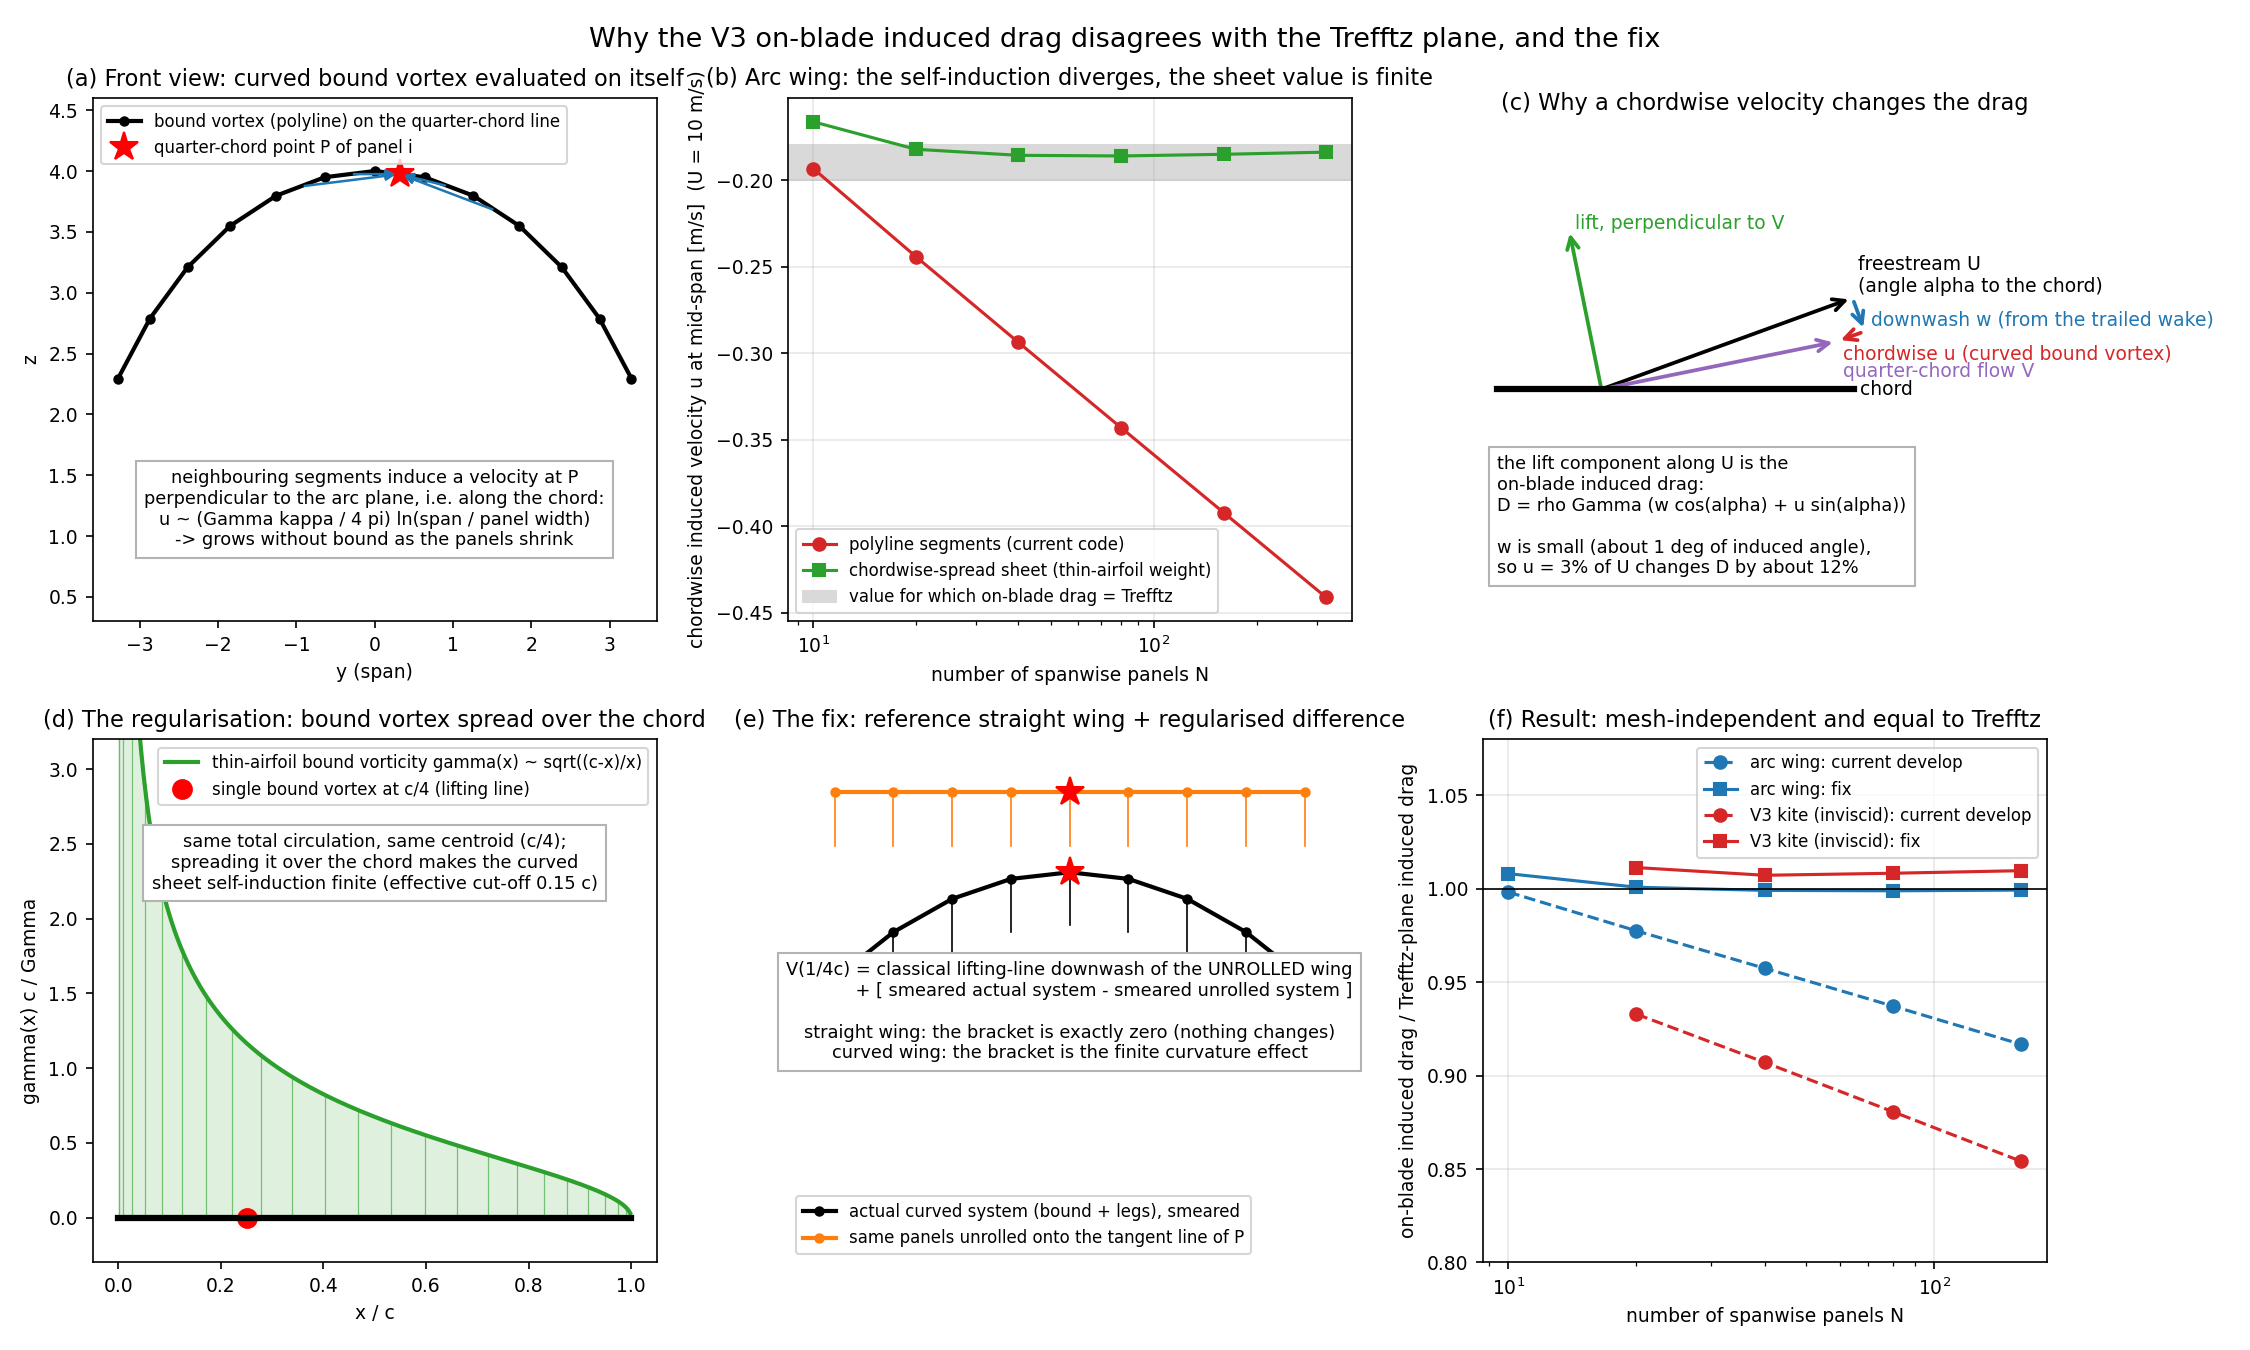
\includegraphics[width=\textwidth]{08_curved_bound_vortex_regularisation.png}
\caption{Mechanism and fix (\texttt{docs/figures/08}). (a) Front view of the curved bound polyline with the quarter-chord point of panel $i$. (b) Arc wing, mid-span: chordwise self-induction from the polyline (grows logarithmically with $N$) and from the chordwise-spread sheet (finite); grey band: value at which on-blade drag equals Trefftz. (c) Why a chordwise velocity changes the drag, eq.~\eqref{eq:drag}. (d) The thin-airfoil bound vorticity distribution used for the regularisation; effective cut-off $\exp\langle\ln|x-c/4|\rangle_\gamma = 0.15\,c$. (e) The unrolled reference construction. (f) Convergence of on-blade over Trefftz drag before and after.}
\label{fig:explain}
\end{figure}

\section{How the literature treats the singularity}
\label{sec:lit}

\subsection{Li, Gaunaa, Pirrung, Ramos-Garc\'ia, Horcas (2020): evaluate at the three-quarter chord}
Reference~\cite{li2020} identifies the LL-P\&S evaluation (bound vortex on its own line, as in Phillips and Snyder~\cite{phillips2000}) as log-singular and demonstrates its mesh dependence numerically (their Figs.~3--4). Their remedy (LL-mod) evaluates the bound-vortex induction at the three-quarter-chord point, subtracts the 2D infinite-vortex induction of the section's own strength, treats the difference as constant along the chord and adds it to the quarter-chord velocity that sets the force direction. The trailed vortices are also evaluated at the three-quarter chord in LL-mod, which they note makes the iteration less stable. This is the reference cited by~\cite{gaunaa2026} for LL-Gaunaa; neither the 2026 paper nor its online appendix~\cite{appendix2026} (results for ten planforms at 120 sections, no convergence study) adds implementation detail.

\emph{Test in the VSM framework.} The recipe was implemented literally: for every panel $j$, the finite bound segment at the control point $\mathbf C_i$ minus (for $j=i$) the infinite line, reused at $\mathbf P_i$. Results (on-blade/Trefftz): straight AR\,8 wing 0.848, straight AR\,4 wing 0.815, arc 0.84, swept--anhedral elliptic wing with perpendicular legs 0.865, swept $30^\circ$ wing $0.50\to0.35$. The straight-wing failure is decisive: for a finite wing with spanwise-varying $\Gamma$ the ``3D minus 2D'' difference at the three-quarter chord is not zero (it contains the finite-span tails and the $\Gamma$-variation of the bound vortex; $+0.02$\,m/s at mid-span and $+0.11$\,m/s near the tips at $U=20$\,m/s on the AR\,8 wing), and eq.~\eqref{eq:drag} amplifies it. The same quantity used for the three-quarter-chord angle of attack, which the VSM has always done, is correct and untouched; only its reuse as a quarter-chord velocity fails. Since~\cite{gaunaa2026} reports LL-Gaunaa within 0.6\,\% of a VLM on straight wings, the authors' implementation must differ from this literal reading, most plausibly by taking ``curved minus straight'' (as first described in~\cite{li2018}) rather than ``3D minus 2D''. This should be confirmed with the authors. In their appendix the on-blade Oswald factor sits 5.6\,\% and 1.1\,\% above the Trefftz one for the 15\,\% and 25\,\% swept wings, within 0.6\,\% for the dihedral, anhedral and combined wings.

\subsection{Reid and Hunsaker (2020), Goates and Hunsaker (2021, 2023): effective lifting line and jointed legs}
References~\cite{reid2020,goates2021,goates2023} (open-source implementation MachUpX) prove that the induced velocity on a lifting line is finite only where the line's second derivative vanishes and the trailing vortices leave it perpendicularly. Their construction: each control point sees an \emph{effective} lifting line, straight (tangent) near the point and blended into the true curve with a Gaussian of prescribed width (``blending distance'', recommended $\gtrsim 25\,\%$ of the span, MachUpX default one semispan); each trailing vortex has a finite \emph{joint} of length $\delta c$ perpendicular to the effective line before turning along the freestream (recommended $\delta\gtrsim0.15$, MachUpX default 0.15). Bound segments of the other sections are kept. Validation is on circulation distributions and $C_L$ of planar swept wings against panel methods and experiment; induced drag and non-planar wings are not examined.

\emph{Test in the VSM framework.} The construction was implemented for the quarter-chord direction velocity, everything else unchanged (Table~\ref{tab:rh}). It is mesh-independent, as claimed, but the induced drag depends on the two lengths, by 17\,\% on the V3 and 12\,\% on the arc across reasonable choices, because the blending distance is precisely the cut-off of the curvature logarithm; the authors' insensitivity statement concerns lift, which is far less sensitive. With streamwise rib legs the swept wing fails (0.2--0.7), since the perpendicular joints no longer represent the vortex system that carries the force.

\begin{table}[h]\centering\small
\caption{Reid--Hunsaker construction in the VSM framework: on-blade over Trefftz drag at $N=80$. Joint length and blending distance in local chords, except the MachUpX column (defaults: joint 0.15\,$c$, blending one semispan). Last column: the regularisation of Section~\ref{sec:fix} at the same $N$.}
\label{tab:rh}
\begin{tabular}{lccccccc}
\toprule
case & 0.25\,/\,1 & 0.5\,/\,1 & 1.0\,/\,1 & 0.5\,/\,0.5 & 0.5\,/\,2 & MachUpX & regularised\\
\midrule
straight AR 8 & 1.000 & 1.000 & 1.000 & 1.000 & 1.000 & 1.001 & 1.000\\
swept $30^\circ$, rib legs & 0.642 & 0.471 & 0.198 & 0.191 & 0.637 & 0.688 & 0.982\\
arc, $R=4c$ & 1.049 & 1.025 & 1.004 & 1.003 & 1.052 & 1.117 & 0.999\\
elliptic, 10\,\% sweep, 25\,\% anhedral & 1.007 & 0.988 & 0.968 & 0.968 & 1.008 & 1.042 & 1.015\\
V3 kite & 1.003 & 0.966 & 0.930 & 0.885 & 1.032 & 1.053 & 1.008\\
\bottomrule
\end{tabular}
\end{table}

\subsection{Other approaches}
\begin{itemize}[nosep]
  \item \emph{Li et al.\ 2018}~\cite{li2018}: correct a straight-blade model by the difference between the curved and an imaginary straight bound vortex. Same subtraction idea as below, but with single filaments, hence mesh dependent; abandoned in~\cite{li2020}.
  \item \emph{Guermond 1990}~\cite{guermond1990}: matched-asymptotic lifting-line theory for curved and swept wings. Shows analytically that the curvature term is finite once the inner (airfoil-scale) problem is accounted for, using Hadamard finite-part integrals. It is the theoretical basis for a chord-scale cut-off but is not a numerical scheme with horseshoes and polars.
  \item \emph{Vortex core on the bound vortex} (e.g.\ QBlade~\cite{qblade}, core radius a fraction of chord): Reid and Hunsaker note these are ``very sensitive to the cutoff/core distance''. Tested here with the code's Vatistas kernel: the projection of an on-line point to the core boundary produces spurious velocities of order $\Gamma/(4\pi\epsilon)$ and unusable results.
  \item \emph{Three-quarter-chord directions} (Weissinger, Ranneberg~\cite{ranneberg2015}, the VSM default before the \texttt{develop} branch): no singularity, but the induced drag is overestimated by 20--40\,\% on the V3~\cite{gaunaa2026}.
  \item \emph{Trefftz-plane drag only} (Ranneberg): exact for the total in steady uniform inflow, unavailable with body rates or distributed inflow, no spanwise distribution.
\end{itemize}

\section{The regularisation implemented on the branch}
\label{sec:fix}

\subsection{Formulation}
Let $\mathbf K^{\mathrm{LL}}_j(\mathbf P)$ denote the induction at $\mathbf P$ of ring $j$ without its bound segment (two legs and two semi-infinite wake filaments; this is what the code's LLT influence matrix holds), and let $\mathbf K^{\mathrm{sheet}}_j(\mathbf P)$ denote the induction of ring $j$ with its bound vorticity and its leg starting points spread along the chord:
\begin{equation}
\mathbf K^{\mathrm{sheet}}_j(\mathbf P)=\sum_{q=1}^{M} w_q\Big[\mathbf K^{\mathrm{seg}}\big(\mathbf n_{2,jq}\to\mathbf n_{1,jq};\mathbf P\big) + \mathbf K^{\mathrm{leg}}\big(\mathbf n_{1,jq}\to\mathbf T_{1,j}\big)+\mathbf K^{\mathrm{leg}}\big(\mathbf T_{2,j}\to\mathbf n_{2,jq}\big)\Big] + \mathbf K^{\mathrm{wake}}_j(\mathbf P),
\end{equation}
where the strip nodes lie on each node's own leg line,
\begin{equation}
\mathbf n_{k,jq} = \mathbf b_{k,j} + \frac{x_q - x_{ac}}{1-x_{ac}}\,(\mathbf T_{k,j}-\mathbf b_{k,j}),\qquad x_{ac}=\tfrac14,
\end{equation}
so that the strip legs are collinear with the actual legs, and the chordwise stations and weights follow the thin-airfoil distribution $\gamma(x)\propto\sqrt{(c-x)/x}$ through $x_q=\sin^2\phi_q$, $w_q\propto\cos^2\phi_q$, $\phi_q=(q-\tfrac12)\pi/(2M)$, $M=24$ (\texttt{thin\_airfoil\_strips}). The distribution has its centroid at $c/4$, so the far field of the sheet equals that of the single filament.

For each evaluation panel $i$, the \emph{unrolled} reference wing is built on the tangent line $\mathbf t_i$ of panel $i$ through $\mathbf P_i$: every node keeps its arc-length coordinate along the bound line, the legs are perpendicular to the line in panel $i$'s chord direction with the panel's own chord length, and the wake keeps its direction. The quarter-chord velocity is then
\begin{equation}
\boxed{\;
\mathbf V_{1/4,i}=\mathbf V_\infty+\sum_j\Gamma_j\Big[\mathbf K^{\mathrm{LL}}_{j,\mathrm{unrolled}(i)}(\mathbf P_i)
+\mathbf K^{\mathrm{sheet}}_{j}(\mathbf P_i)-\mathbf K^{\mathrm{sheet}}_{j,\mathrm{unrolled}(i)}(\mathbf P_i)\Big].\;}
\label{eq:fix}
\end{equation}
The first term is Prandtl's classical downwash of the straight wing with the actual $\Gamma(s)$, exact for straight wings (ratio 1.000). The bracket is the curvature, sweep and skew effect; it is identically zero on a straight wing with perpendicular legs, finite because both sheets regularise the near field at the chord scale, and convergent because no filament is evaluated on its own line. The semi-infinite wake filaments cancel identically between the actual and unrolled systems, so the wake model plays no role. Nothing else changes: the three-quarter-chord magnitude (which already contains the LL-mod term of~\cite{li2020}), the circulation map, the AT force and the wake are untouched. The single-filament limit of the bracket recovers the curved-minus-straight idea of~\cite{li2018}; the chordwise spreading is the discrete counterpart of the inner solution in~\cite{guermond1990}; the local straightening is the mechanism of~\cite{reid2020} without its two empirical lengths. The effective cut-off implied by the distribution is $\exp\langle\ln|x-c/4|\rangle_\gamma=0.1515\,c$; the number of strips does not matter beyond $M\approx 20$ (24 and 32 strips give the same arc self-induction to three digits). Implementation: \texttt{assemble\_curved\_bound\_correction\_AIC} in \texttt{src/VSM/core/utils.py}, called once per solve from \texttt{BodyAerodynamics.update\_effective\_angle\_of\_attack\_if\_VSM}; about 1\,s at 80 panels.

\subsection{Verification against the Trefftz plane}

\begin{table}[h]\centering\small
\caption{On-blade over Trefftz-plane induced drag with eq.~\eqref{eq:fix}, inviscid polars (\texttt{curved\_bound\_vortex\_validation.py}).}
\label{tab:fix}
\begin{tabular}{lccccc}
\toprule
case & $N=10$ & 20 & 40 & 80 & 160\\
\midrule
straight rectangular, AR 8 & -- & -- & 1.000 & 1.000 & --\\
straight, ribs skewed $22^\circ$ & -- & -- & 1.029 & 1.030 & --\\
swept $30^\circ$, streamwise ribs & -- & -- & 0.971 & 0.982 & 0.988\\
circular arc, $110^\circ$, $R=4c$ & 1.008 & 1.001 & 0.999 & 0.999 & 0.999\\
elliptic, 10\,\% sweep, 25\,\% anhedral, rib legs & -- & -- & 1.014 & 1.015 & 1.017\\
elliptic, same, perpendicular legs & -- & -- & 1.024 & 1.024 & --\\
V3 kite, rib legs & -- & 1.011 & 1.007 & 1.008 & 1.010\\
V3 kite, perpendicular legs & -- & -- & 1.042 & 1.038 & --\\
\bottomrule
\end{tabular}
\end{table}

Two residuals remain and are unrelated to the bound vortex: the swept wing converges to 0.99 rather than 1.00, and the straight wing with skewed ribs sits at 1.03 with or without the fix. Both point to the attached-trailed force on non-perpendicular legs and are a separate, smaller item. The 4\,\% excess with perpendicular legs on the V3 is likewise not caused by the bound-vortex term (it is the same with the bound segments on the line).

\subsection{Rib versus perpendicular legs}
\label{sec:legs}
The September choice of rib legs was made with the singular bound-on-line term. Table~\ref{tab:legs} repeats the comparison with eq.~\eqref{eq:fix} in place (\texttt{leg\_direction\_study.py}). Perpendicular legs are built per node from the mean span-perpendicular chord direction of the two adjacent panels, with length $(1-a)\bar c$ from the bound point; the control point, frame and chord are the CP1 ones in both cases.

\begin{table}[h]\centering\small
\caption{Rib against perpendicular legs, attached-trailed (AT) force on and off, $N=80$. Top: on-blade over Trefftz induced drag, inviscid polars. Bottom: V3 viscous polars (CAD geometry, 2D RANS polars, 50 panels) against RANS~\cite{poland2026} at $1$--$13^\circ$.}
\label{tab:legs}
\begin{tabular}{lcccc}
\toprule
 & rib, AT on & rib, AT off & perp., AT on & perp., AT off\\
\midrule
circular arc, $110^\circ$, $R=4c$ & 0.999 & 0.946 & 0.999 & 0.946\\
elliptic, 10\,\% sweep, 25\,\% anhedral & 1.015 & 0.974 & 1.025 & 1.002\\
V3 kite, $10^\circ$ & 1.008 & 0.917 & 1.038 & 0.994\\
swept $30^\circ$, kinked at the root & 0.982 & 0.980 & NaN & NaN\\
\midrule
V3 mean $|\Delta C_L|$ & 0.020 & 0.017 & 0.031 & 0.037\\
V3 mean $|\Delta C_D|/C_D$ & 3.0\,\% & 1.4\,\% & 3.8\,\% & 2.3\,\%\\
\bottomrule
\end{tabular}
\end{table}

On the arc the ribs are perpendicular and the two coincide; there the AT force is required (0.946 to 0.999). On the elliptic wing and the V3 both the AT contribution ($+0.04$ and $+0.09$ with ribs, $+0.02$ and $+0.04$ with perpendicular legs) and the remainder depend on the leg direction, and their sum is within 1.5\,\% of the Trefftz plane with ribs but 2.5--4\,\% high with perpendicular legs. Dropping the AT force with perpendicular legs gives 1.00 on those two wings but 0.946 on the arc, so no rule is consistent on all three. The excess with perpendicular legs is not a bound-vortex effect (Table~\ref{tab:fix} shows it with the bound segments on the line as well); it is a property of chordwise legs on a swept quarter-chord line, where the leg carries a Kutta--Joukowski force from the downwash with a streamwise component. The authors' results on swept wings differ from the Trefftz plane by a similar amount but in the opposite direction: for the swept--anhedral elliptic wing, Table~2 of~\cite{gaunaa2026} gives $e_{\mathrm{Osw,Blade}}=1.101$ against $e_{\mathrm{Osw,Trefftz}}=1.080$ for LL-Gaunaa, i.e.\ on-blade induced drag 1.9\,\% \emph{below} the Trefftz plane, and their VLM reference is 2.8\,\% below (1.106 against 1.075); the appendix~\cite{appendix2026} gives 5\,\% and 1\,\% below for the 15\,\% and 25\,\% swept wings. The authors read this as a limitation of the Trefftz-plane analysis for curved wings. Note also that~\cite{gaunaa2026} (Section~3) runs the chordwise legs ``up to the trailing edge'', whereas the perpendicular legs tested here have the fixed length $(1-a)\bar c$ and end on the trailing edge only where it is parallel to the quarter-chord line; the paper states explicitly that the leg direction ``is not specified by theoretical results'' and ``is effectively a modeling choice''. On the V3 the perpendicular legs also lower the inviscid lift from 0.639 to 0.600 (the fixed-length leg at the curved tips ends far from the trailing edge), which moves the viscous $C_L$ away from RANS at every angle below $10^\circ$. On the kinked swept wing they cannot be built. The rib legs are therefore kept: constructible on every input planform, within 1.5\,\% of the far-wake drag on all curved cases, and the best V3 agreement with RANS (within 3\,\% in $C_D$ up to $10^\circ$; the 13$^\circ$ point, 10\,\% high, is near the RANS stall).

\subsection{Independent evidence: the arc self-induction}
On the arc the chordwise self-induction that makes on-blade equal Trefftz is $u\approx-0.19$\,m/s (interpolating between the trailed-only value, ratio 1.079 at $u=0$, and the on-line value at $N=80$, ratio 0.951 at $u=-0.34$\,m/s). The chordwise-spread sheet gives $u=-0.186$\,m/s at every $N$ from 40 to 320 (Figure~\ref{fig:explain}b). Nothing was tuned to obtain this agreement.

\subsection{Effect on the V3 kite polars}
Figure~\ref{fig:polars} and Table~\ref{tab:polars} show the V3 (CAD geometry, 2D RANS polars at Re $5\times10^5$, 50 panels, 2.82\,m/s) with the old three-quarter-chord directions, the quarter-chord directions with the bound segments on the line and the regularisation, against RANS~\cite{poland2026} and the wind-tunnel data of Poland et al.~\cite{poland2026}. Lift is unchanged; the drag rises by a fraction of the induced drag, most at high lift and in sideslip, and lands on the RANS values up to $10^\circ$.

\begin{table}[h]\centering\small
\caption{V3 kite drag coefficient, $\beta=0$.}
\label{tab:polars}
\begin{tabular}{cccccc}
\toprule
$\alpha$ & old 3/4-chord & bound on the line & regularised & RANS (Re $10^6$) & wind tunnel (Re $5\times10^5$)\\
\midrule
$5^\circ$ & 0.061 & 0.054 & 0.055 & 0.052 ($4^\circ$) & 0.076 ($5.4^\circ$)\\
$7^\circ$ & 0.075 & 0.063 & 0.065 & 0.064 & 0.090 ($7.3^\circ$)\\
$9^\circ$ & 0.094 & 0.074 & 0.079 & 0.084 ($10^\circ$) & 0.107 ($9.4^\circ$)\\
$13^\circ$ & 0.148 & 0.110 & 0.120 & 0.110 & 0.217 ($13.4^\circ$)\\
\bottomrule
\end{tabular}
\end{table}

\begin{figure}[p]\centering
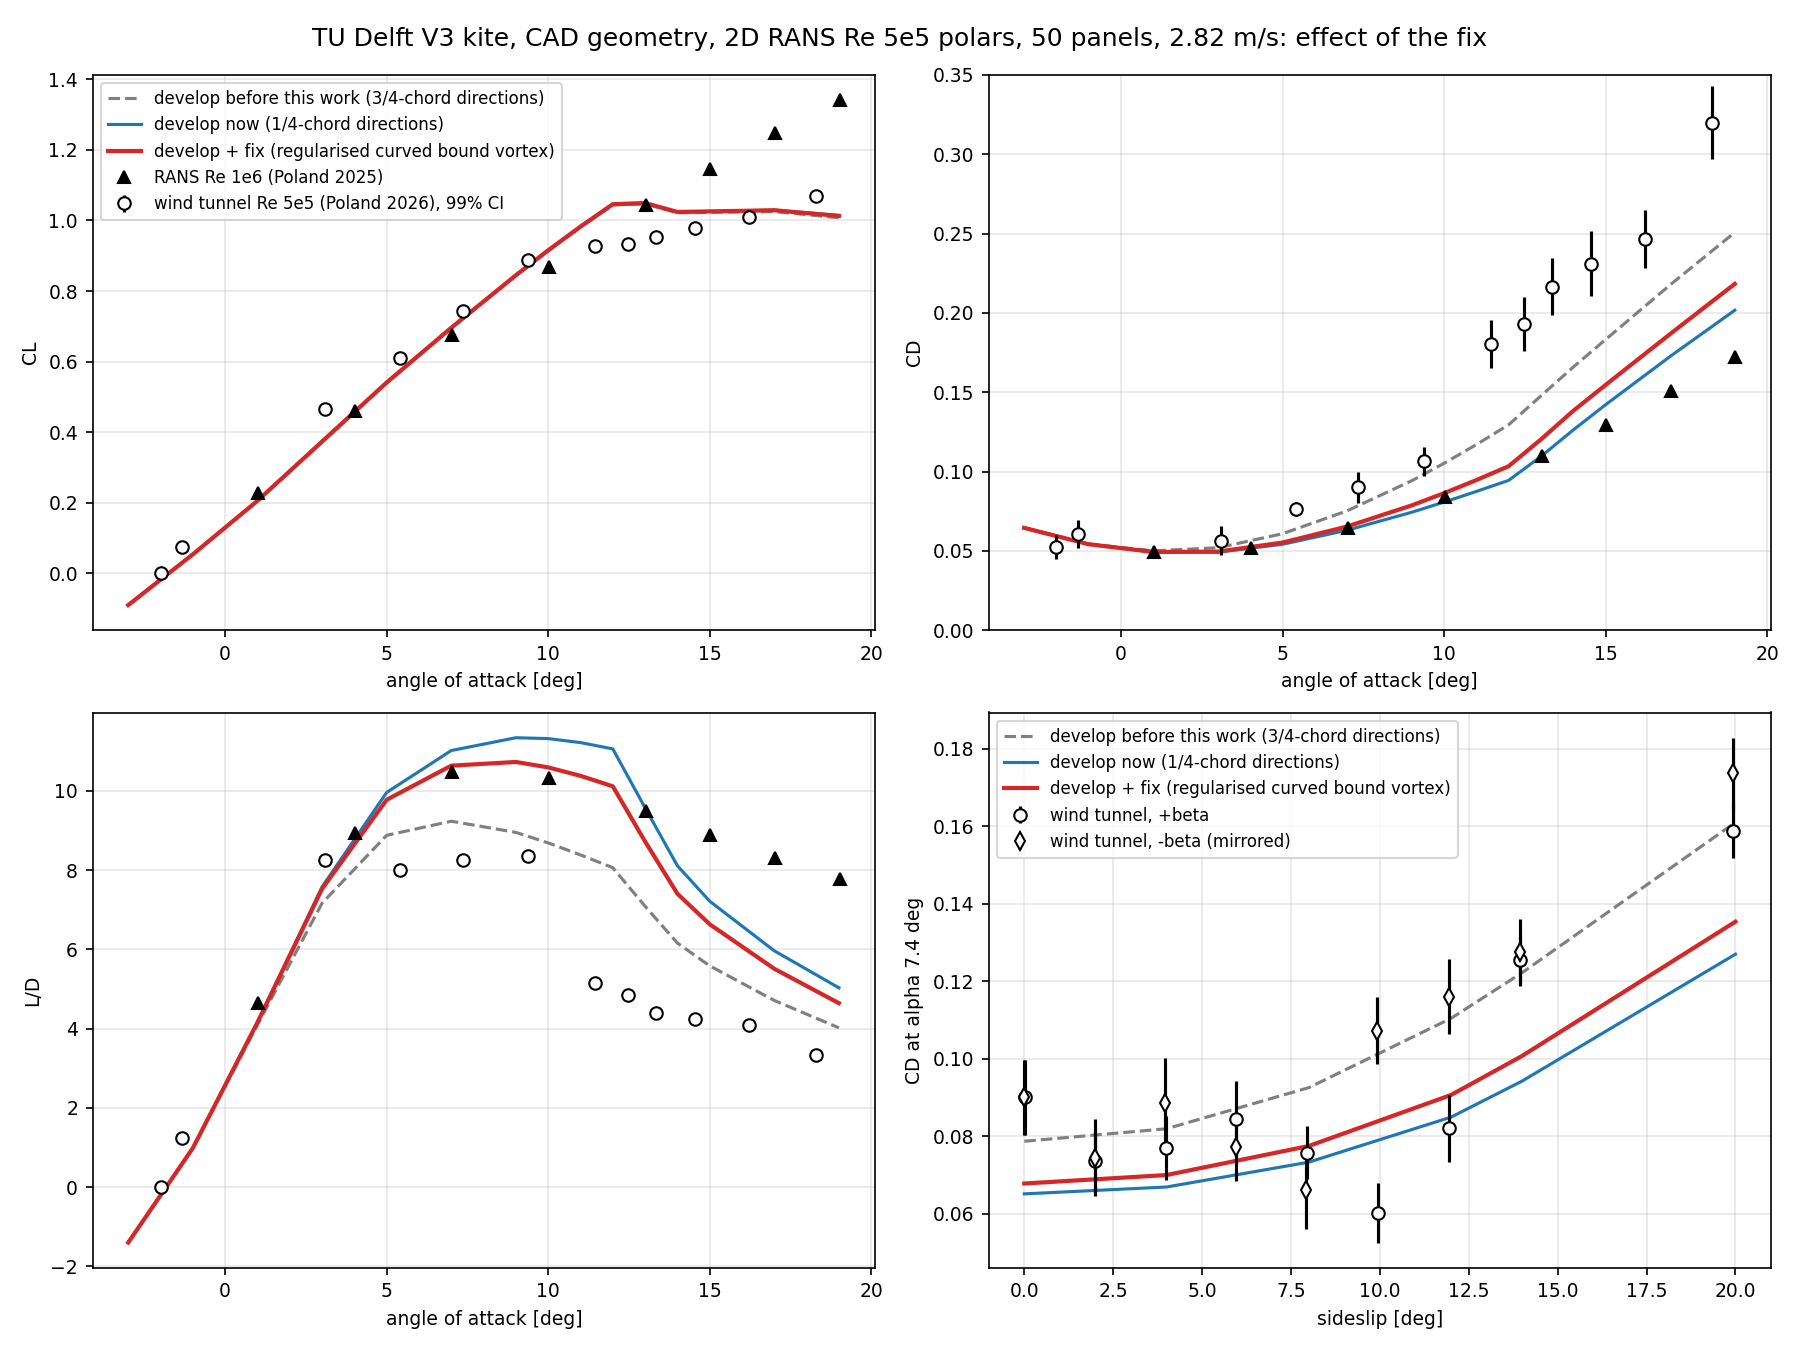
\includegraphics[width=\textwidth]{09_v3_polars_curved_bound_vortex_fix.png}
\caption{V3 kite polars (\texttt{docs/figures/09}) with the old three-quarter-chord directions, the quarter-chord directions with the bound segments on the line, and the regularisation, against RANS and the wind-tunnel data of Poland et al.\ (1:6.5 rigid model, no bridles, open-jet corrections applied).}
\label{fig:polars}
\end{figure}

The remaining gap to the wind tunnel is lift-dependent, $\Delta C_D\approx0.003+0.037\,C_L^2$, and is shared by RANS ($C_D=0.043+0.052\,C_L^2$ versus $0.041+0.085\,C_L^2$ measured). Poland et al.\ attribute it to the 3--4\,mm model canopy, the flow behind the leading-edge tube and transition. It is not a lifting-line issue and the fix is not meant to close it; the old three-quarter-chord directions appeared to close part of it only because they overestimate the induced drag by 20--40\,\%.

\section{Assessment and open items}
\begin{itemize}[nosep]
  \item The mechanism of the fix (straighten locally, regularise the legs, keep the far field) is that of Reid and Hunsaker~\cite{reid2020}; the difference-form goes back to Li et al.~\cite{li2018}. The contribution here is the replacement of the two empirical lengths by the thin-airfoil chordwise distribution, which fixes the cut-off at $0.15\,c$ from theory, and the demonstration that this yields Trefftz-consistent induced drag on curved kites. It should be presented as such, with~\cite{reid2020,li2020,guermond1990} cited.
  \item To be confirmed with the authors of~\cite{gaunaa2026,li2020}: how the curved bound-vortex influence is applied at the quarter chord in their code, and how it behaves when the number of sections is doubled.
  \item Open: the attached-trailed force on legs that are skewed or swept with respect to the flow (swept wing 0.99, skewed ribs 1.03, perpendicular legs on the swept V3 and elliptic lines 1.025--1.04, Section~\ref{sec:legs}). The leg direction itself stays with the ribs (Section~\ref{sec:legs}). Not quantified: the section polars are rib-section polars while CP1 applies them in the span-perpendicular plane.
\end{itemize}

\begin{thebibliography}{99}\small
\bibitem{gaunaa2026} M.~Gaunaa, A.~Li, G.~R.~Pirrung, From thin airfoil theory to finite wings: consistent implementation of Lifting Line-based models, J.\ Phys.: Conf.\ Ser.\ 3224 (2026) 042030.
\bibitem{appendix2026} M.~Gaunaa, A.~Li, G.~R.~Pirrung, Internet appendix for ``From thin airfoil theory to finite wings'', Zenodo, doi:10.5281/zenodo.18222326 (2026).
\bibitem{li2026} A.~Li, M.~Gaunaa, G.~R.~Pirrung, K.~L{\o}nb{\ae}k, Relaxation limits and artificial viscosity for lifting line methods, TORQUE 2026.
\bibitem{li2020} A.~Li, M.~Gaunaa, G.~R.~Pirrung, N.~Ramos-Garc\'ia, S.~G.~Horcas, The influence of the bound vortex on the aerodynamics of curved wind turbine blades, J.\ Phys.: Conf.\ Ser.\ 1618 (2020) 052038.
\bibitem{li2018} A.~Li, G.~Pirrung, H.~Aa.~Madsen, M.~Gaunaa, F.~Zahle, Fast trailed and bound vorticity modeling of swept wind turbine blades, J.\ Phys.: Conf.\ Ser.\ 1037 (2018) 062012.
\bibitem{reid2020} J.~T.~Reid, D.~F.~Hunsaker, A general approach to lifting-line theory, applied to wings with sweep, J.\ Aircraft 58 (2021), doi:10.2514/1.C035994.
\bibitem{goates2021} C.~D.~Goates, D.~F.~Hunsaker, Practical implementation of a general numerical lifting-line method, AIAA SciTech 2021, paper 2021-0118.
\bibitem{goates2023} C.~D.~Goates, D.~F.~Hunsaker, Modern implementation and evaluation of lifting-line theory for complex geometries, J.\ Aircraft (2023), doi:10.2514/1.C036748. Code: \url{https://github.com/usuaero/MachUpX}.
\bibitem{guermond1990} J.-L.~Guermond, A generalized lifting-line theory for curved and swept wings, J.\ Fluid Mech.\ 211 (1990) 497--513.
\bibitem{phillips2000} W.~F.~Phillips, D.~O.~Snyder, Modern adaptation of Prandtl's classic lifting-line theory, J.\ Aircraft 37 (2000) 662--670.
\bibitem{ranneberg2015} M.~Ranneberg, Direct wing design and inverse airfoil identification with the nonlinear Weissinger method, arXiv:1501.04983 (2015).
\bibitem{qblade} QBlade documentation, Lifting line free vortex wake, \url{https://docs.qblade.org/src/theory/aerodynamics/lifting_line/lifting_line.html}.
\bibitem{poland2026} J.~A.~W.~Poland, J.~M.~van Spronsen, M.~Gaunaa, R.~Schmehl, Wind tunnel load measurements of a leading-edge inflatable kite rigid-scale model, Wind Energ.\ Sci.\ 11 (2026) 911.
\end{thebibliography}

\end{document}
